\documentclass[t]{beamer}

\usepackage[ngerman]{babel}
\usepackage[utf8]{inputenc}
\usepackage{amssymb}
\usepackage{amsmath}
\usepackage{amsthm}
\usepackage{amsfonts}
\usepackage{setspace}
\usepackage{tikz}
\usepackage{lmodern}

\usetheme{Madrid}
\usecolortheme{default}
\date{\today}

\title{Simulating Visual Geometry}
\author{Patrick Bayer}
\linespread{1.5}

\begin{document}
	%Titelseite
	\begin{frame}
		\titlepage
	\end{frame}

	%Inhaltsverzeichnis
	\begin{frame}{Inhalt}
		\tableofcontents
	\end{frame}

	\section{Konstruktion eines Simulationsnetzes}
	\begin{frame}{Konstruktion eines Simulationsnetzes}
		\textcolor{blue}{Input:}	
		\begin{itemize}
			\item Beliebiges Netz zur Visualisierung bestehend aus drei- oder viereckigen Elementen
			\item Meistens nicht zur Simulation geeignet
			\item Physikalische Eigenschaften des Objektes (Materialdicke, \dots)
		\end{itemize}
		\textcolor{blue}{Idee:}
			\begin{itemize}
					\item Konvexe Formen als Primitive für das Simulationsnetz
			\end{itemize}
		\end{frame}

	\begin{frame}{Konstruktion eines Simulationsnetzes}
		\begin{columns}
			\column{0.5\textwidth}
				\centering
				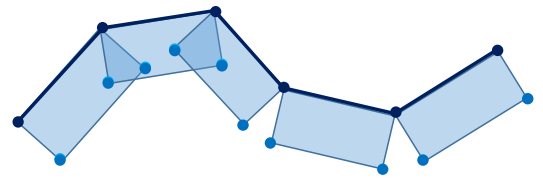
\includegraphics[scale = 0.4]{PhysicalMeshCreation_Step1.png}\\
				(1) Elemente werden nach innen extrudiert.\\
				$\Rightarrow$ volumetrische, konvexe Primitive
			
			\column{0.5\textwidth}
					\centering
					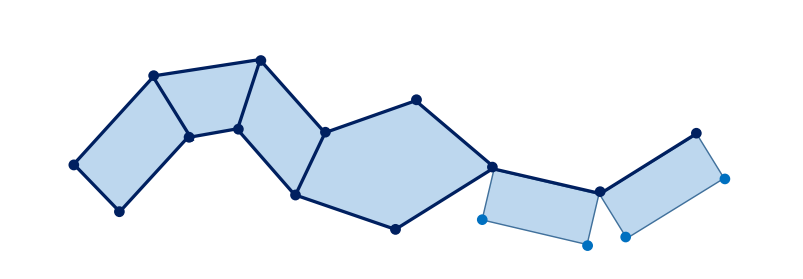
\includegraphics[scale = 0.31]{PhysicalMeshCreation_2}\\
					(2) Bereits vorhandene konvexe Formen werden direkt in Primitive transformiert
		\end{columns}
	\end{frame}
		
	\begin{frame}{Konstruktion eines Simulationsnetzes}
		\textcolor{blue}{Verbinden der Primitive:}
		\begin{itemize}
			\item Graph mit Primitiven als Knoten und Verbindungen als Kanten
			\item Ausgangssituation: Ruhelage des Objektes
			\item Zwei Primitive sind verbunden $\Leftrightarrow$ Die Primitive berühren oder überlappen sich
		\end{itemize}
	\end{frame}

	\begin{frame}{Konstruktion eines Simulationsnetzes}
		\textcolor{blue}{Verbinden von Subnetzen:}
		\begin{itemize}
			\item Verwendung von Joints definiert durch Boxen
			\item Ball joint, Hinge-Joint, Slider Joints
		\end{itemize}
		\vfill
		\centering
		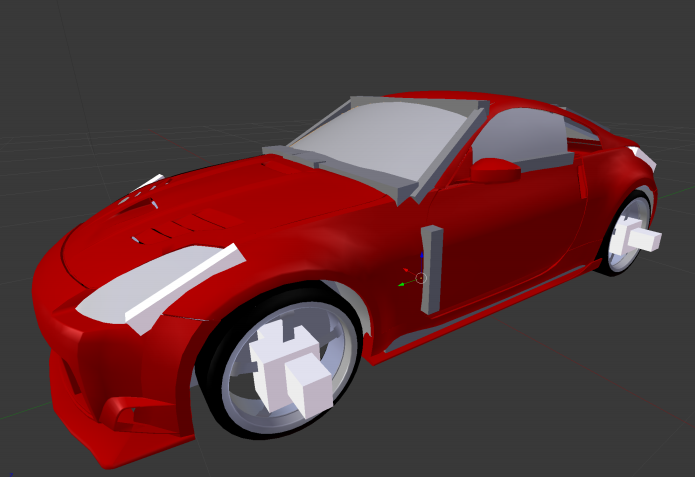
\includegraphics[scale = 0.3]{Joints.png}
	\end{frame}
	
	\section{Die Simulationsmethode}
	\begin{frame}{Die Simulationsmethode}
		\begin{itemize}
			\item \textbf{Oriented particle method}
			\item Geometrisch motiviert
			\item Einfach und schnell
			\item Partikel haben neben den linearen Attributen (Position, Geschwindigkeit) eine Rotation und Winkelgeschwindigkeit
			\item Basiert auf Shape Matching und Position Based Dynamics
		\end{itemize}
	\end{frame}	
	
	\begin{frame}{Die Simulationsmethode}
		\textcolor{blue}{Shape Matching:}
		\begin{itemize}
			\item Simulation von Elastizität
			\item Arbeitet mit Partikeln ohne Verbindungen
		\end{itemize}
		\begin{center}
			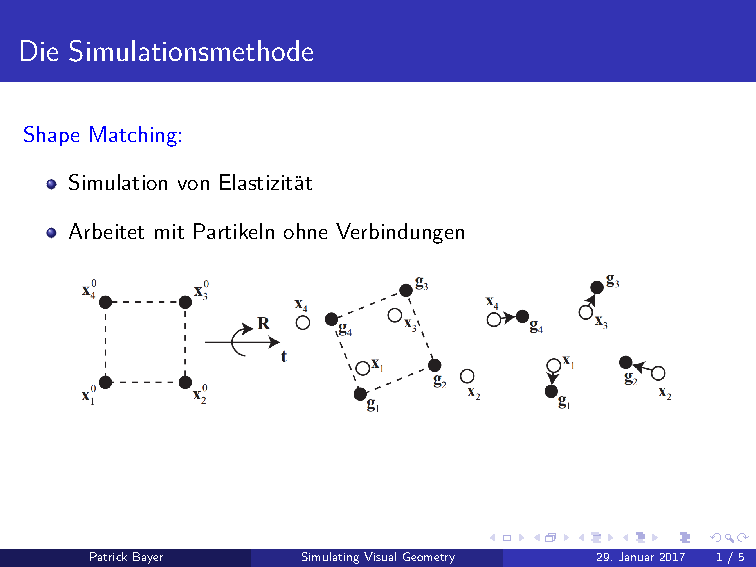
\includegraphics[scale = 0.25]{ShapeMatching.png}
		\end{center}
		
	\end{frame}

	
	
	\begin{frame}{Die Simulationsmethode}
		\textcolor{blue}{Generalized Position Based Dynamics}
		\begin{itemize}
			\item Integrationsmechanismus zur Simulation von Partikeln
			\item Partikel haben eine Position \textbf{x}, eine Geschwindigkeit \textbf{v}, eine Rotation \textbf{q} und eine Winkelgeschwindigkeit $\omega$
			\item Schritt 1: Vorhersage von \textbf{x} und \textbf{q}
					\begin{center}
						$\mathbf{x}_p \leftarrow \mathbf{x}+\mathbf{v}\Delta \mathbf{t}$
					\end{center}
					\begin{center}
						$\mathbf{q}_p \leftarrow [\frac{\mathbf{\omega}}{\vert \mathbf{\omega \vert}} sin(\frac{\vert \omega \vert \Delta \mathbf{t}}{2}), cos(\frac{\vert \omega \vert \Delta \mathbf{t}}{2})]\mathbf{q}$
					\end{center}
			\item Schritt 2: Korrektur der Positionen $\mathbf{x}_p$ anhand gegebener Zwangsbedingungen
		\end{itemize}
	\end{frame}
	
	\begin{frame}{Die Simulationsmethode}
		\begin{itemize}
			\item Schritt 3: Update von \textbf{x}, \textbf{v}, \textbf{q}, $\mathbf{\omega}$
				\begin{center}
					$\mathbf{v} \leftarrow \frac{\mathbf{x}_p - \mathbf{x}}{\Delta \mathbf{t}}$
				\end{center}
				\begin{center}
					$\mathbf{x} \leftarrow \mathbf{x}_p$
				\end{center}
					\begin{center}
					$\mathbf{q} \leftarrow \mathbf{q}_p$
				\end{center}
				\begin{center}
					$\omega \leftarrow \frac{axis(\mathbf{q}_p \mathbf{q}^{-1})*angle(\mathbf{q}_p \mathbf{q}^{-1})}{\Delta \mathbf{t}}$
				\end{center}
		\end{itemize}
	\end{frame}

	\begin{frame}{Die Simulationsmethode}
		\textcolor{blue}{Collision Handling:}
		\begin{itemize}
			\item Finde Überschneidungen von Objektgrenzen
			\item Identifiziere alle beteiligten Primitive und prüfe für jedes Paar, ob eine Kollision auftritt
			\item Seperating Axis Theorem
		\end{itemize}	
	\end{frame}
	
	\section{Deformation der Primitive}
	
	\begin{frame}{Deformation der Primitive}
		\begin{itemize}
			\item Oriented Particle Method führt zu visuellen Fehlern (Lücken, \dots)
		\end{itemize}
		\begin{center}
			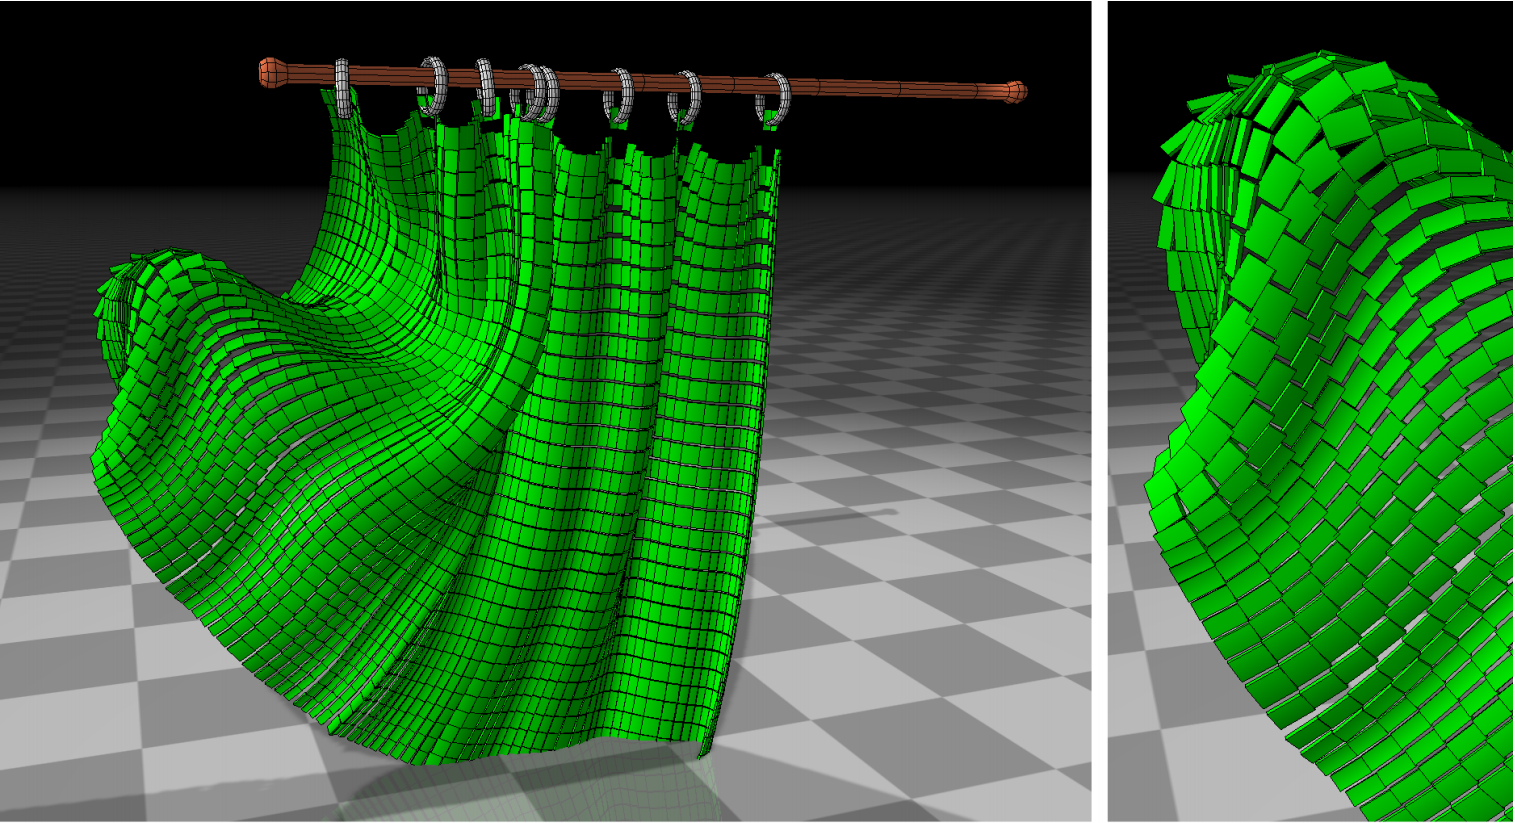
\includegraphics[scale = 0.25]{Curtain_1.png}
		\end{center}
	\end{frame}

	\begin{frame}{Deformation der Primitive}
		\begin{itemize}
			\item Konvexe Eigenschaft der Primitive muss erhalten bleiben
					$\Rightarrow$ Nutze die Local Affine Deformation Matrix $\mathbf{A}$
					\begin{center}
						$\mathnormal{\mathbf{A}}=\sum\limits_{\mathnormal{i}}(\mathnormal{\mathbf{A}_i}+\mathnormal{\mathbf{m}_i \mathbf{x}_i \mathbf{\bar{x}}_i^T})-M\mathnormal{\mathbf{x}_{cm} \mathbf{\bar{x}}_{cm}^T}$ \\
						$\mathnormal{\mathbf{A}_{i}}=\frac{1}{5}mr^2\mathbf{R}_\mathnormal{i}$
					\end{center}
			\item Berechne die Deformationsmatrix \textbf{D}
				\begin{center}
					$\mathnormal{\mathbf{D}}=\mathnormal{\mathbf{A \bar{A}^{-1}}}$ \\
					$\mathbf{\bar{A}}=\sum\limits_{\mathnormal{i}}(\mathnormal{\mathbf{\bar{A}}_i+\mathbf{m}_i\mathbf{\bar{x}}_i\mathbf{\bar{x}}_i^T})-M\mathnormal{\mathbf{\bar{x}}_{cm} \mathbf{\bar{x}}_{cm}^T}$
				\end{center}
				\begin{center}
					$\mathnormal{\mathbf{A}_{i}}=\frac{1}{5}mr^2\mathbf{I}$
				\end{center}
		\end{itemize}
	\end{frame}
	
	\section{Das Visualisierungsnetz}
	\begin{frame}{Das Visualisierungsnetz}
		\begin{center}
			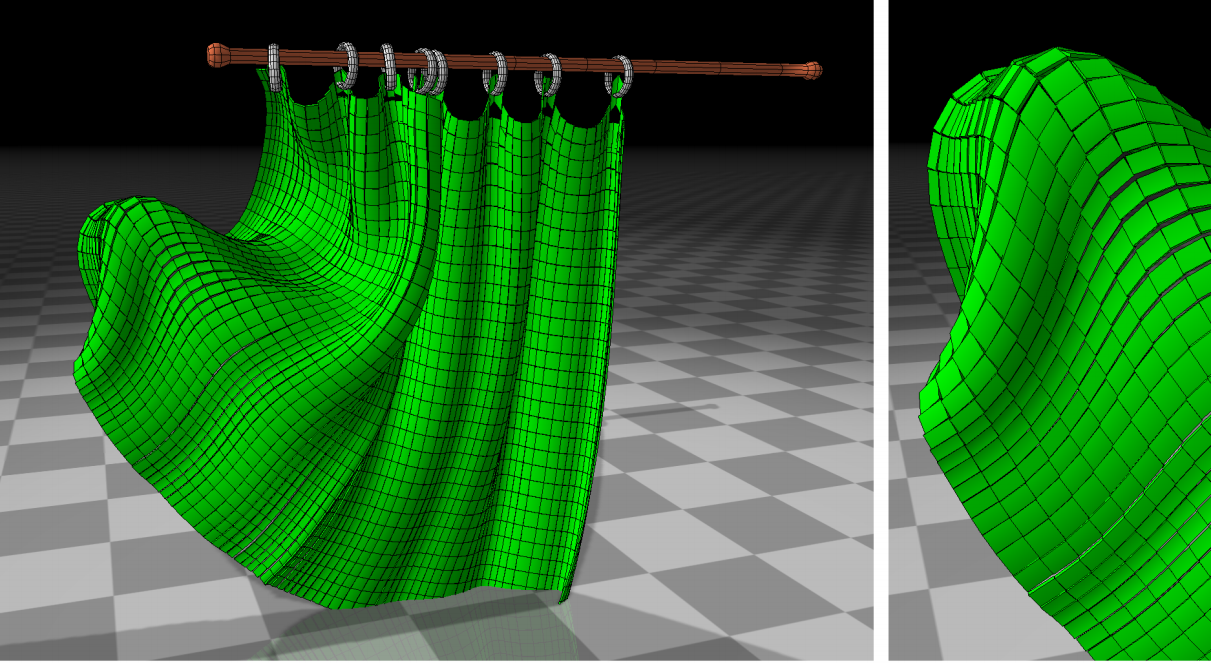
\includegraphics[scale = 0.275]{Curtain_2.png}
		\end{center}
		\begin{itemize}
			\item Auch nach der Deformation der Primitive sind kleine Lücken zu finden
		\end{itemize}
	\end{frame}
	
	\begin{frame}{Das Visualisierungsnetz}
		\begin{minipage}{0.5\textwidth}
			\begin{itemize}
				\item Gruppiere die Eckpunkte der Primitive nach ihren Positionen
				\item Berechne den Durchschnitt der Positionen
				\item Die visuelle Position aller beteiligten Primitive ist der Durchschnitt der Positionen
			\end{itemize}
		\end{minipage}\begin{minipage}{0.5\textwidth}
			\centering
			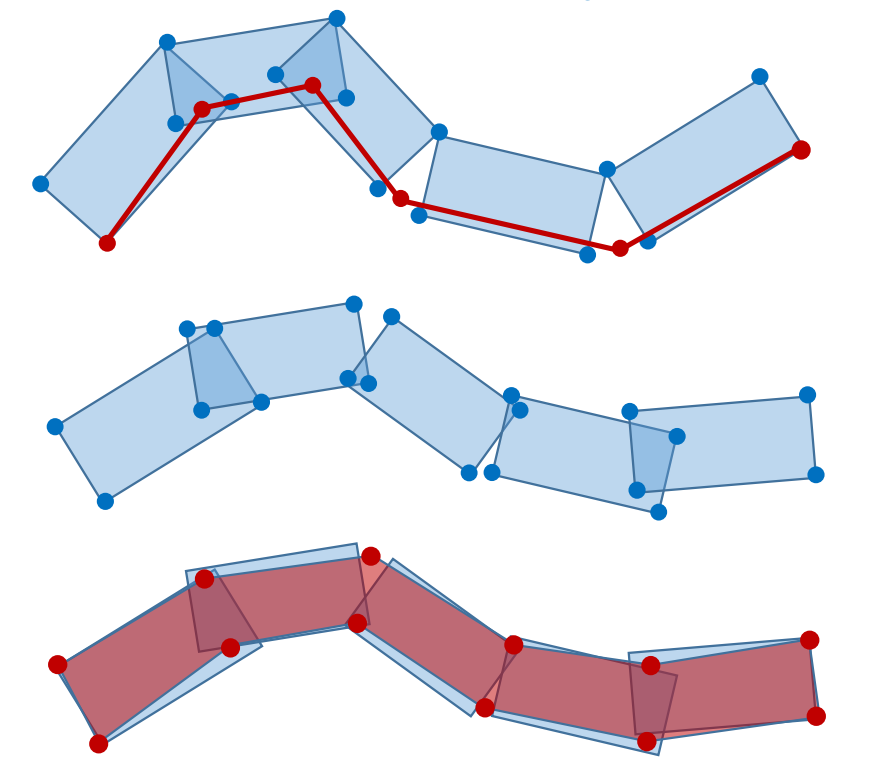
\includegraphics[scale = 0.25]{PhysicalMeshCreation_Step234.png}
		\end{minipage}
	\end{frame}
	
	\section{Plastische Deformation}
	\begin{frame}{Plastische Deformation}
		\begin{itemize}
			\item Behandle Objekte wie Starrkörper bis eine Deformation eintritt
			\item Schwellenwert für die Geschwindigkeit an den Kontaktpunkten
			\item Deformationsoffset = Geschwindigkeit * Time Step Size
			\item Primitive, die nach einer Deformation einen Joint überschneiden, werden als fix betrachtet
		\end{itemize}
	\end{frame}
	
	\section{Brüche und Risse}
	\begin{frame}{Brüche und Risse}
		\textcolor{blue}{Trennbrüche:}
		\begin{itemize}
			\item Menge von verbundenen konvexen Polyedern als Bruchmuster bestehend aus Bruchzellen
		\end{itemize}
			\begin{minipage}{0.6\textwidth}
				\begin{itemize}
					\item Finde Überschneidungen der Objektgrenzen mit dem Bruchmuster und alle beteiligten Primitive\\
					$\Rightarrow$ Neues, unabhängiges Objekt bestehend aus allen Primitiven innerhalb einer Zelle 
				\end{itemize}
			\end{minipage}\begin{minipage}{0.4\textwidth}
				\begin{center}
					\centering
					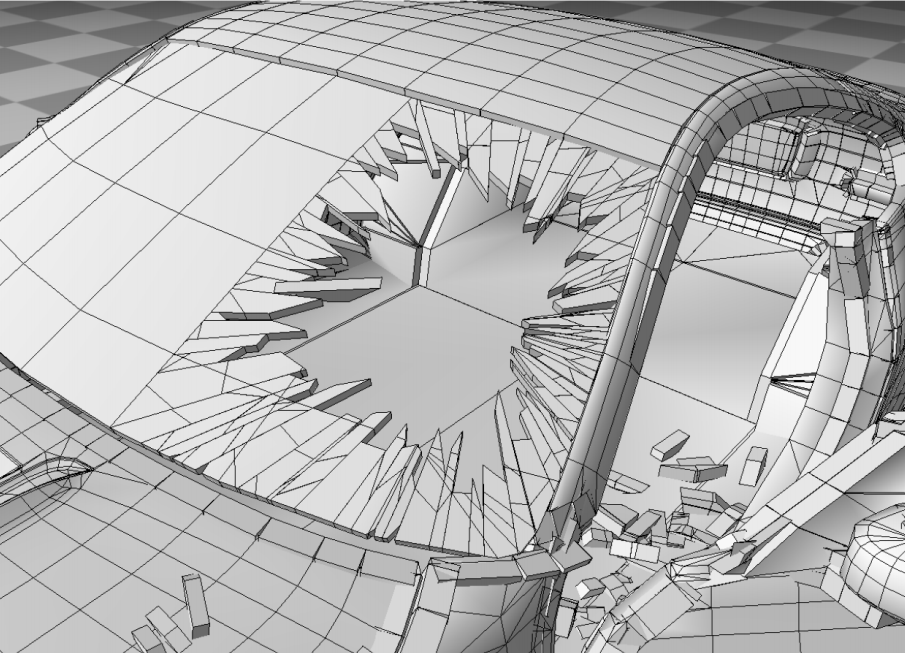
\includegraphics[scale = 0.2]{GlassFracture.png}
				\end{center}
			\end{minipage}
	\end{frame}

	\begin{frame}{Brüche und Risse}
		\textcolor{blue}{detaillierte Deformation:}
		\begin{minipage}{0.5\textwidth}
			\begin{itemize}
				\item Behalte alle resultierenden Teile nach einem Bruch in demselben Objekt\\
				$\Rightarrow$ Das verfeinerte Netz erlaubt detaillierte Deformationen
			\end{itemize}
		\end{minipage}\begin{minipage}{0.5\textwidth}
			\centering
			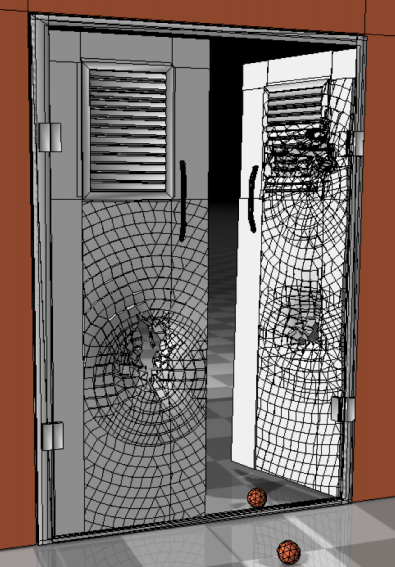
\includegraphics[scale = 0.35]{Door1.png}
	\end{minipage}

	\end{frame}
	
	\begin{frame}{Brüche und Risse}
		\textcolor{blue}{Verformungsbrüche und Risse:}
		\begin{itemize}
			\item Schwellenwert für die Distanz zwischen zwei Primitiven zur Identifizierung von Brüchen und Rissen
			\item Nutzer kann Risslinien vordefinieren, indem nur eine Teilmenge der Verbindungen erlaubt ist zu reißen
		\end{itemize}
	\end{frame}

	\begin{frame}{Brüche und Risse}
		\textcolor{blue}{Visualisierung von Brüchen:}
		\begin{itemize}
			\item Das Bruchmuster wird im nicht deformierten Zustand ausgerichtet\\
				$\Rightarrow$ Sowohl die alten als auch die neuen Primitive erhalten dieselbe \textit{id}
		\end{itemize}
		\begin{center}
			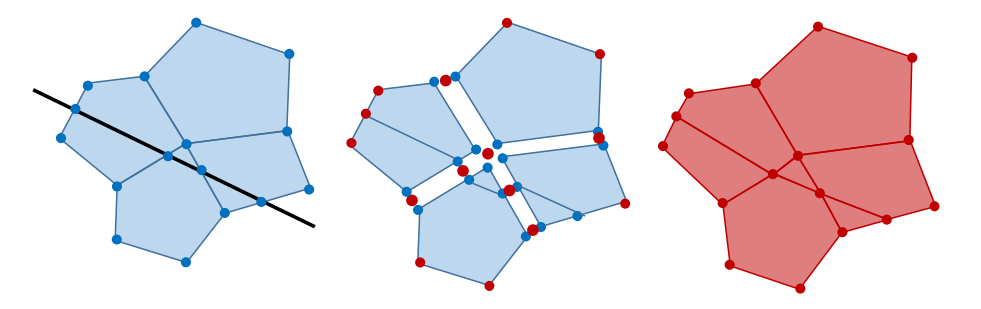
\includegraphics[scale = 0.4]{Fracture.png}
		\end{center}
	\end{frame}
	
	\begin{frame}{Brüche und Risse}
		\textcolor{blue}{Visualisierung von Rissen:}
		\begin{itemize}
			\item Berechne \textit{val(id)} als Anzahl der Primitive mit derselben \textit{id}
			\item Besuche alle Nachbarn mit derselben \textit{id} im Verbindungsgraphen
			\item Falls die Anzahl der besuchten Eckpunkte kleiner als \textit{val(id)} ist, ist ein Riss aufgetreten
			\item Die besuchten Eckpunkte erhalten eine neue \textit{id}
		\end{itemize}
	\end{frame}

	\begin{frame}{Brüche und Risse}
		\centering
		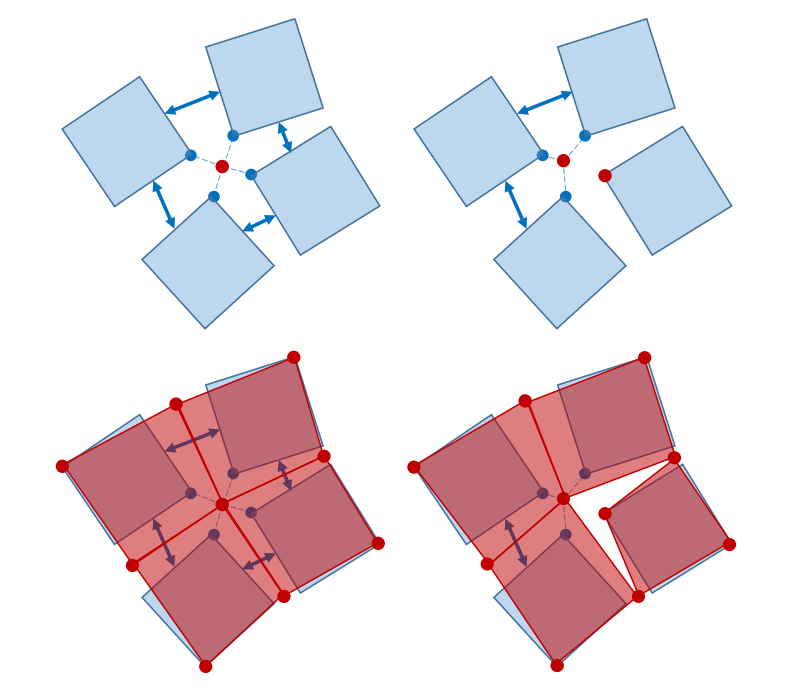
\includegraphics[scale = 0.35]{Tearing.png}
	\end{frame}
	
	\begin{frame}{Zusammenfassung}
		\begin{itemize}
			\item Methode zur Simulation und Visualisierung von Deformationen, Brüchen und Rissen in Echtzeit-Anwendungen
			\item Simulationsnetz, das direkt aus einem beliebigen Visualisierungsnetz hervor geht
			\item Konvexe Polyeder als Primitive
			\item Oriented Particle Method
		\end{itemize}
	\end{frame}

	\begin{frame}{Literaturverzeichnis}
		Alle Informationen und Bilder stammen aus folgenden Quellen:
		\begin{itemize}
			\item Matthias Müller, Nuttapong Chentanez, Miles Macklin: Simulating Visual Geometry, Proceedings of the 9th International Conference on Motion in Games, 2016
			\item MÜLLER M., CHENTANEZ N.: Solid simulation with oriented particles. ACM Trans. Graph. 30, 4 (July 2011), 92:1–92:10
			\item MÜLLER M., HEIDELBERGER B., TESCHNER M.: Meshless deformations based on shape matching. In Proc. SIGGRAPH 2005 (2005), pp. 471–478
		\end{itemize}
	\end{frame}
\end{document}